
\section{Methodology}

Our method for checking what operating system a host is using involved an analysis of packets. By analyzing the first packet of a TCP session, we can make a good guess of the operating system based on a few attributes of the packet in the header information.

\subsection{Packet Analysis}

Our OS fingerprinting technique relies on the TCP/IP protocol suite.  With the TCP/IP protocol suite, we are able to transfer a data payload over the network.  The payload is encapsulated within a TCP segment, and, in turn, encapsulated in an IP datagram \cite{tcpip}.  Both levels of encapsulation include a header with information.  IP header information includes items such as version, TTL, source and destination IP; and TCP header information includes TCP window size, source and destination port \cite{header}. Figures \ref{fig:ipDiagram} and \ref{fig:tcpDiagram} give a graphical representation of a IP and TCP headers, respectively.

\begin{figure}
\centering
\begin{minipage}{.5\textwidth}
  \centering
  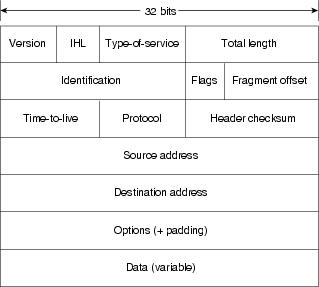
\includegraphics[width=.8\linewidth]{images/tcpdiagram.jpg}
  \captionof{figure}{IP Datagram Header~\cite{Cisco1}}
  \label{fig:ipDiagram}
\end{minipage}%
\begin{minipage}{.5\textwidth}
  \centering
  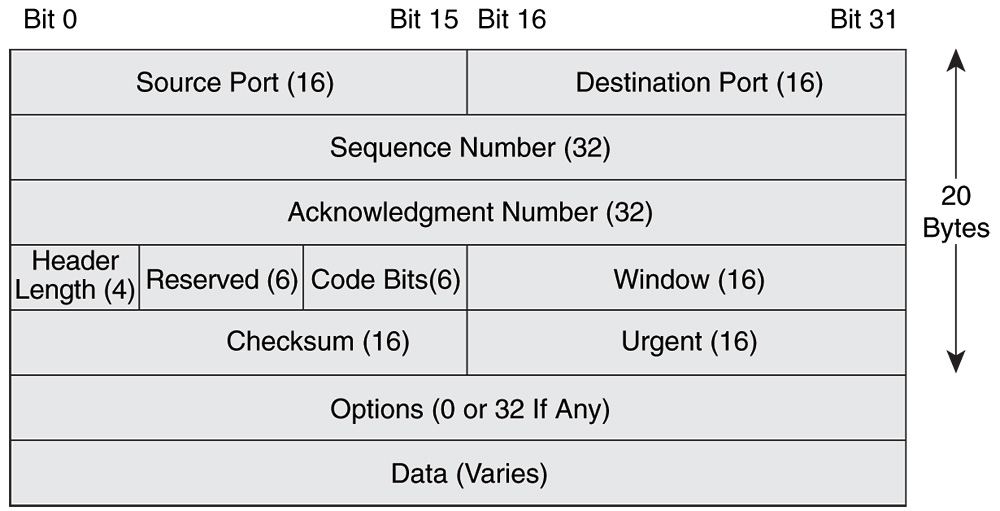
\includegraphics[width=1\linewidth]{images/tcpheader.jpg}
  \captionof{figure}{TCP Segment Header~\cite{tcpheader1}}
  \label{fig:tcpDiagram}
\end{minipage}
\end{figure}

\subsubsection{Window Size}

The TCP window size is an option set in the TCP header.  It sets an initial byte size for informing the client that it is to only accept that many bytes at one time.  Microsoft defines the TCP window size as ``the amount of receive data (in bytes) that can be buffered at one time on a connection. The sending host can send only that amount of data before waiting for acknowledgments for data sent and window updates from the receiving host'' \cite{Microsoft1}. 

All Operating Systems behave differently and choose a different initial number of bytes for their TCP Window Size in the TCP three-way handshake.  We can use this disparity to identify the OS that we are attempting to establish a connection with.  This is assuming, of course, that the default OS values have not been changed.  All values are typically user-defined, but it is often the case that an administrator leaves these values at the OS defaults, which is why we are able to identify an OS based on this value.


\subsubsection{Time to Live}

``Time-to-live (TTL) is a value in an Internet Protocol (IP) packet that tells a network router whether or not the packet has been in the network too long and should be discarded.'' ~\cite{Rouse07}.  Each Operating System begins with a TTL that is decremented after each ``hop'' (i.e., a visit to a router). Figure \ref{fig:ipDiagram} shows the TTL field is specified before the protocol field.  Because this value is constantly changing it can be very difficult, even useless, to use this method alone in identifying the OS of the machine in question.  However, when used along with the TCP window size, we are able to differentiate between two different Operating Systems that use the same initial TCP window size but different TTL values.

In Figure \ref{fig:osFunction}, we depict some Python code which returns a guess as to which OS we may have established a connection to.  We pass along both the TCP window size and the TTL of a packet retrieved from an established connection. The function first looks at the TCP window size, and in most cases, returns a guess based on just that.  A few values of TCP window size, however, check the TTL afterward.  For example, if we look at Windows 2003 Server and OpenBSD, we notice that both operating systems use a TCP windows size of 16384, but because Windows 2003 Server uses a TTL of 128, we are able to determine based on this TTL value if it is Windows 2003 Server and not OpenBSD. This approach works in most situations but if the number of hops between an OS fingerprinter and the server were to exceed 64 hops, our tool would incorrectly identify a Windows 2003 Server OS as an OpenBSD OS.  

\begin{figure}
	\center{\fbox{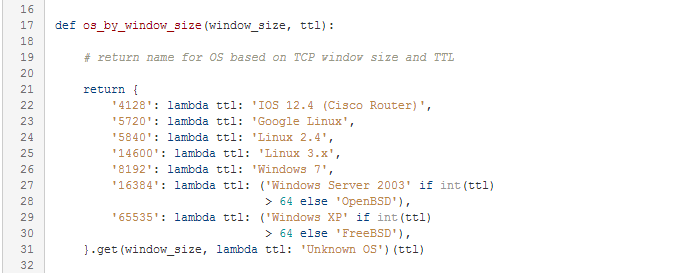
\includegraphics[width=.9\textwidth]
	{images/code2.png}}}
	\caption{\label{fig:osFunction} OS Identifier Function}
\end{figure}

\subsection{Implementation}

For our implementation, we chose to use the high-level programming language Python \cite{Python} and for a packet manipulation tool with a Python wrapper, we chose to use Scapy \cite{Scapy}.  We chose Python because it is both very human readable (in comparison to other programming languages), cross-platform (i.e., will run on Windows as well as Linux), and contains a wide range of tools and libraries available for us to utilize.  Scapy adds the functionality needed to establish TCP connections, assemble TCP and IP packets, as well as to analyze the packet headers, which is needed for our OS fingerprinting technique.

\begin{figure}
	\center{\fbox{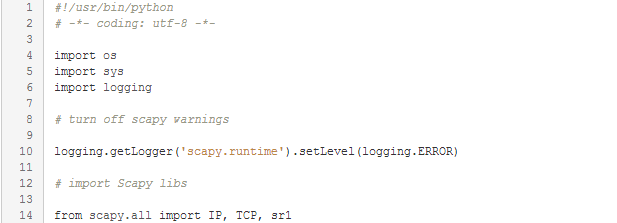
\includegraphics[width=.9\textwidth]
	{images/code1.png}}}
	\caption{\label{fig:setupCode} Setup Code}
\end{figure}

In Figure \ref{fig:setupCode}, we import the necessary libraries and extensions needed for execution of our tool. Scapy is a verbose tool, so we turned off any unneeded warning or information messages from being displayed but kept critical error messages.  Scapy also include a wide array of functionality which is well beyond the scope of our project, so we imported only what we needed.  Since we are dealing with header information from TCP and IP headers, we imported the TCP and IP modules from Scapy; and, since we need a send and receive functionality, we import the ``sr1'' module from Scapy as well.  All this should provide us with the necessary functionality to properly implement a simple OS fingerprinting tool.

\begin{figure}
	\center{\fbox{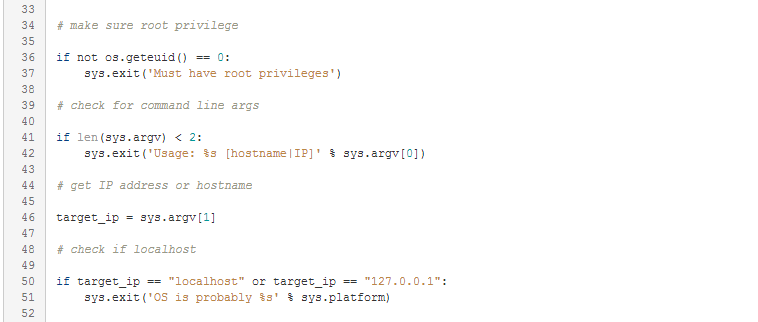
\includegraphics[width=.9\textwidth]
	{images/code3.png}}}
	\caption{\label{fig:prepare} Input and System Checks}
\end{figure}

All tools that take user input should have some input validation, so in Figure \ref{fig:prepare}, we ensure that the user has passed a hostname or IP.  And, since Scapy requires root privileges to craft and analyze packet, we also ensure that the user is executing the tool with the proper privileges needed before continuing execution.

\begin{figure}
	\center{\fbox{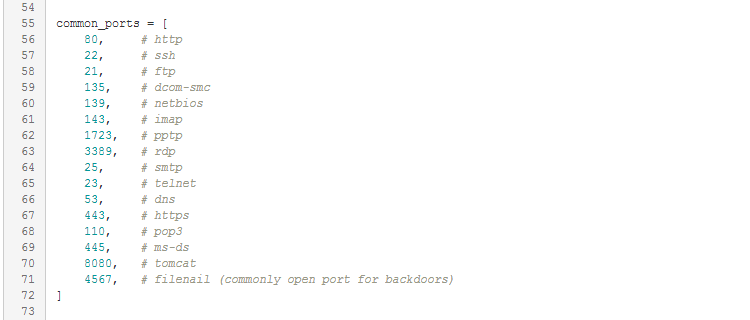
\includegraphics[width=.9\textwidth]
	{images/code4.png}}}
	\caption{\label{fig:ports} Array of Ports}
\end{figure}

A requirement of our tool is that an open port on the target machine is needed in order to establish a connection.  Because it can be very time-consuming to scan every possible port, we chose to only attempt to establish connections on the most commonly open ports we acquired from speedguide.net's security scan of open ports \cite{commonports}. In Figure \ref{fig:ports}, you see the 16 ports we chose to include in our scans.  Although we included 16 ports, we often found in testing that one of the first 6 was almost always open.

\begin{figure}
	\center{\fbox{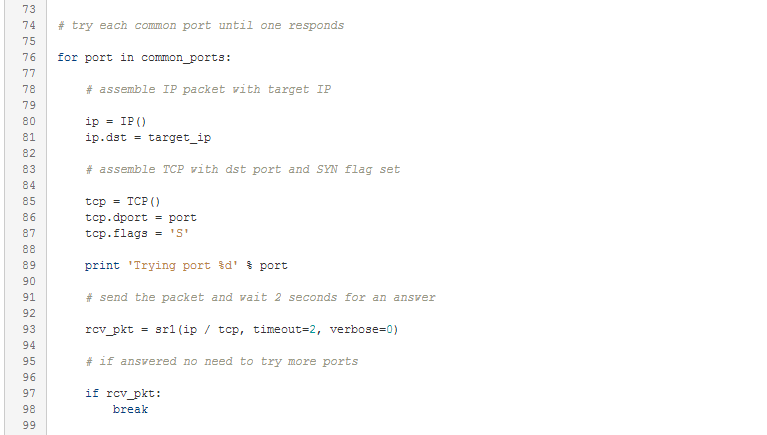
\includegraphics[width=.9\textwidth]
	{images/code5.png}}}
	\caption{\label{fig:loop} Packet Sending Loop}
\end{figure}

In Figure \ref{fig:loop}, you see where most of the Scapy tools were used.  The application iterates through each of the possible ports until a useful packet is received.  An IP header is generated with the target IP, and a TCP header is generated with the specified port number and SYN flag set (in order to initiate a three-way handshake).  These headers are combined and sent to the target machine, as seen on line number 93.  After a packet is sent, the application waits for two seconds for a response and quits the loop if successful or tries the next port if not.

\begin{figure}
	\center{\fbox{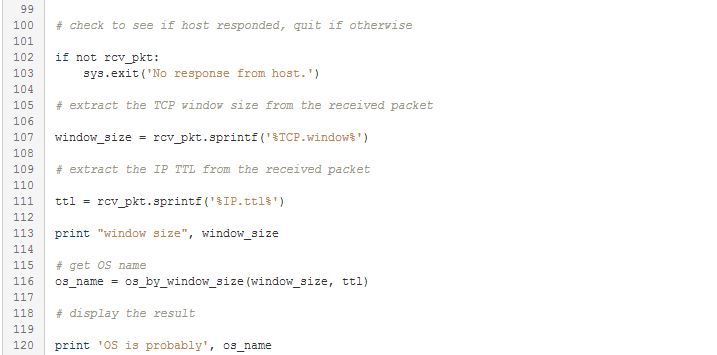
\includegraphics[width=.9\textwidth]
	{images/code6.png}}}
	\caption{\label{fig:results} Result Interpretation and Output}
\end{figure}

Once a packet available for analysis, we can extract the necessary information for OS identification. In Figure \ref{fig:results}, we extract the TTL and TCP window size and pass it to the function we described earlier.  We then print the output of that function and quit.  If the TTL and TCP window size matches one of the defined values, we will have a match, otherwise ``Unknown OS'' is printed to the screen.

\subsection{Testing}

Figure \ref{fig:testScript} shows the shell script we used to test the program.  Because it can be tedious to type out each test case individually, our shell script runs the commands for us with each host we tested.  Some production servers were included in this script but were removed from this paper to maintain the privacy of the server administrators.

\begin{figure}
	\center{\fbox{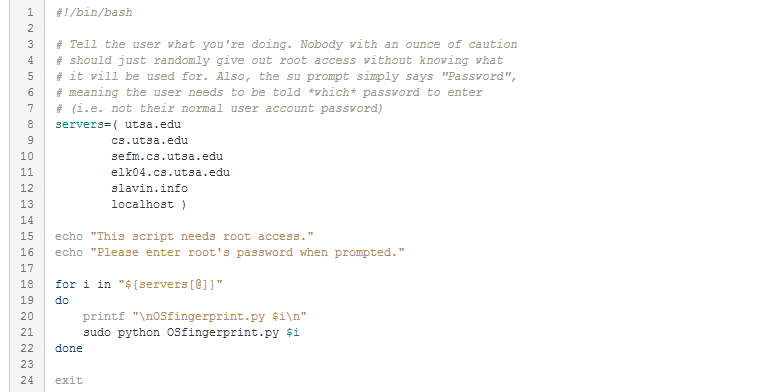
\includegraphics[width=.9\textwidth]
	{images/testCode.png}}}
	\caption{\label{fig:testScript} Testing Shell Script}
\end{figure}

\subsection{Threats To Validity}

As we described earlier, our tool relies on a few assumptions.  Firstly, we must be able to connect to the machine and establish a connection via an open port.  If we are unable to find an open port, we are not able to initiate a three-way handshake and will not be able to analyze the packets needed to determine the OS type.  Secondly, we assume that the OS we are connecting to uses the default values for TCP Window Size and TTL.  If an administrator were to change the default values, our tool could possibly misidentify the OS or print ``Unknown OS''. Finally, specific to the OSs that rely on both TTL and TCP window size, if the number of hops exceeds 64, the OS will be misidentified.  